\section{Tercer captura: Red local muy chica}
Se realizó una tercer captura en una red local que poseía solamente tres hosts mediante el sniffer implementado por nosotros. La captura duró aproximadamente veinte minutos. En este caso vamos a analizar ambas fuentes de información.
En este experimento se tuvo una red con tres hosts, uno es el router (192.168.1.1), otro es dónde se estaba ejecutando la herramienta de monitoreo (192.168.1.124) mientras que en el equipo restante se estuvo realizando una descarga durante casi todo el tiempo (192.168.1.129).
\subsection{Resultados y análisis}
En el gráfico de barras en el que se compara la información de cada símbolo la fuente S con la entropía de la misma se puede ver que, al igual que en los demás experimentos hubo muchísimos más paquetes broadcast que unicast, aún así el valor de la entropía está bastante cerca de ser el óptimo, el cual es 0.5 ya que son dos símbolos.

\subsection{Conclusiones}



\begin{figure}[h]
  \begin{subfigure}{.5\textwidth}
    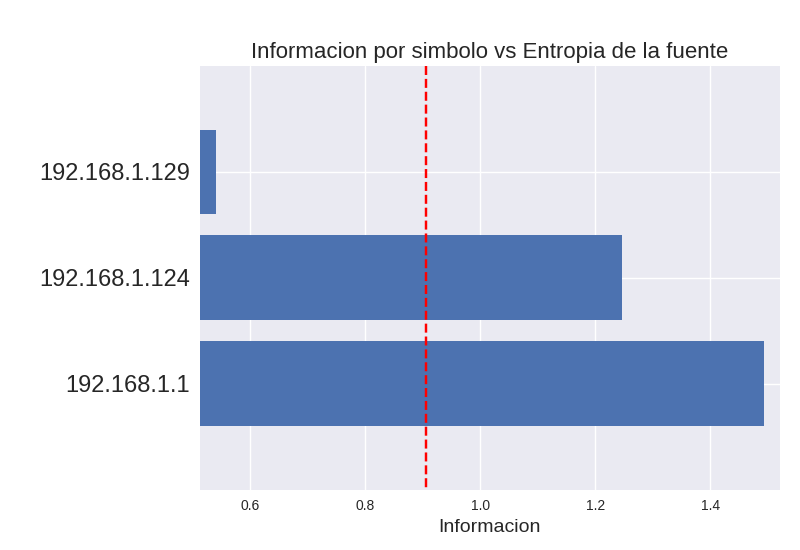
\includegraphics[width=\textwidth]{imagenes/mini_red/mini_red_hosts.png}
  \end{subfigure}
  \label{fig:exp3_hosts_infovsentro}
  \caption{Información de cada símbolo (host) comparada con el valor de la entropía de la fuente de información (red local).}
\end{figure}


\begin{figure}[h]
  \begin{subfigure}{.5\textwidth}
    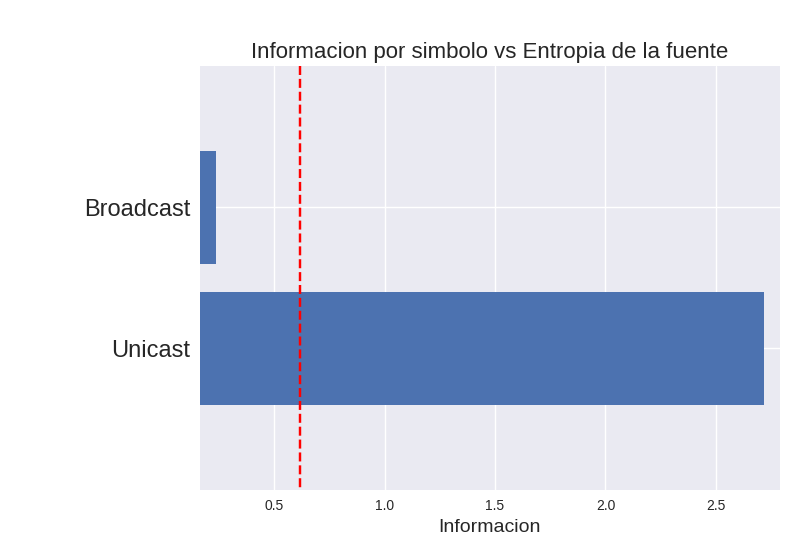
\includegraphics[width=\textwidth]{imagenes/mini_red/mini_red_unicastvsbroadcast.png}
  \end{subfigure}
  \label{fig:exp3_univsbr_infovsentro}
  \caption{Información de cada símbolo (Broadcast / Unicast) comparada con el valor de la entropía de la fuente de información (red local).}
\end{figure}

